\documentclass[../main.tex]{subfiles}
\begin{document}

\section{Modelos}

Para recrear los resultados pasados debemos tomar en cuenta que se utilizó el modelo con mejores resultados, se especifica en su artículo (Chapman et al., 2022) que las características principales  de sus modelos seleccionados son sostenibilidad para implementarlo con datos de nivel y flujo escalares, disponibilidad en herramientas conocidas de ciencia de datos como Weka (Frank et al., 2016), SciKit Learn (Buitinck et al., 2013), and R (R Core Team, 2016) y por ultimo modelos utilizados en otros casos similares, el modelo que seleccionamos fue:

\begin{itemize}
    \item Random Forest Regression (RFR)
\end{itemize}

Ya contando con el modelo pasado se identificaron modelos similares a los anteriores para comparar el desempeño de ambos. 

\begin{itemize}
    \item Modelo de regresión linear
    \item Modelo de regresión Ridge
    \item Modelo de regresión Lasso
    \item Modelo de regresión K-Nearest Neighbor (KNN)
    \item Modelo de regresión con arbol de decision
\end{itemize}

Estos modelos se implementaron por su simplicidad, tanto como gran desempeño en trabajos de colinealidad y por la posibilidad de obtener mejores resultados para compararlos.

Cada modelos requería de dos versiones, una que estimara el nivel del agua (stage) y otro que estimara su flujo (discharge), por lo que al dividirlo por estaciones obtuvimos 48 versiones (12 por temporada), lo cual aplicamos a los modelos con mejor precisión.

Al utilizar las imágenes se realizaron dos pruebas, recortar imágenes para mostrar el área del flujo por la presa y el nivel del agua y aplicar un filtro de escalas grises como fuentes (Figure 3) se manejaron otros modelos especializados, ayudando a relacionar las imágenes con sus respectivos valores en los sensores.  La esperanza es que este mismo modelo pueda identificar con solo la imagen los valores ya sea del nivel del agua tanto como el del flujo. El modelo específico para imágenes fue:

-Modelo de red convulsionar

Todos los modelos y sus resultados están accesibles en el repositorio del proyecto, anexado en este escrito.


\begin{figure}[h]
\centering
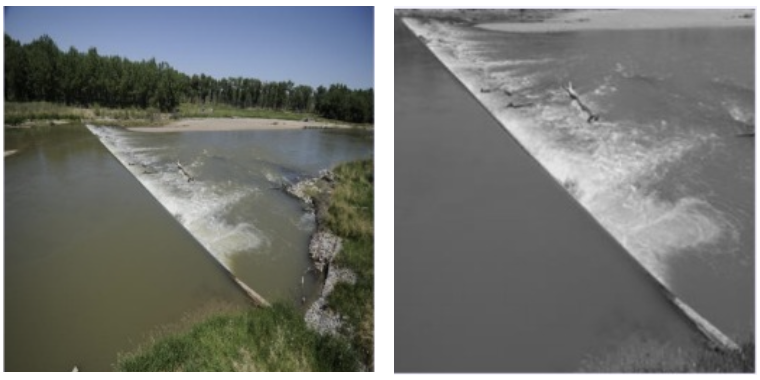
\includegraphics[width=0.8\textwidth]{Fig3}
\caption{Comparación entre imagen original e imagen utilizada con un recorte y filtro de escala de grises.}
\end{figure}


\end{document}
\clearpage